\documentclass[xcolor={dvipsnames}]{beamer}
%\usepackage[utf8]{inputenc}
\usetheme{Madrid}
%\usetheme{Malmoe}
\usecolortheme{beaver}
%\usecolortheme{rose}

%-------------------------------------------------------------------------------
%          -Packages nécessaires pour écrire en Français et en UTF8-
%-------------------------------------------------------------------------------
\usepackage[utf8]{inputenc}
\usepackage[frenchb]{babel}
\usepackage[T1]{fontenc}
\usepackage{lmodern}
\usepackage{textcomp}

%-------------------------------------------------------------------------------

%-------------------------------------------------------------------------------
%                          -Outils de mise en forme-
%-------------------------------------------------------------------------------
\usepackage{hyperref}
\hypersetup{pdfstartview=XYZ}
\usepackage{enumerate}
\usepackage{graphicx}
%\usepackage{multicol}
%\usepackage{tabularx}

%\usepackage{anysize} %%pour pouvoir mettre les marges qu'on veut
%\marginsize{2.5cm}{2.5cm}{2.5cm}{2.5cm}

\usepackage{indentfirst} %%pour que les premier paragraphes soient aussi indentés
\usepackage{verbatim}
%\usepackage[table]{xcolor}  
%\usepackage{multirow}
\usepackage{ulem}
%-------------------------------------------------------------------------------


%-------------------------------------------------------------------------------
%                  -Nécessaires pour écrire des mathématiques-
%-------------------------------------------------------------------------------
\usepackage{amsfonts}
\usepackage{amssymb}
\usepackage{amsmath}
\usepackage{amsthm}
\usepackage{tikz}
\usepackage{xlop}
\usepackage[output-decimal-marker={,}]{siunitx}
%-------------------------------------------------------------------------------


%-------------------------------------------------------------------------------
%                    - Mise en forme 
%-------------------------------------------------------------------------------

\newcommand{\bu}[1]{\underline{\textbf{#1}}}


\usepackage{ifthen}


\newcommand{\ifTrue}[2]{\ifthenelse{\equal{#1}{true}}{#2}{$\qquad \qquad$}}

\newcommand{\kword}[1]{\textcolor{red}{\underline{#1}}}


%-------------------------------------------------------------------------------



%-------------------------------------------------------------------------------
%                    - Racourcis d'écriture -
%-------------------------------------------------------------------------------

% Angles orientés (couples de vecteurs)
\newcommand{\aopp}[2]{(\vec{#1}, \vec{#2})} %Les deuc vecteurs sont positifs
\newcommand{\aopn}[2]{(\vec{#1}, -\vec{#2})} %Le second vecteur est négatif
\newcommand{\aonp}[2]{(-\vec{#1}, \vec{#2})} %Le premier vecteur est négatif
\newcommand{\aonn}[2]{(-\vec{#1}, -\vec{#2})} %Les deux vecteurs sont négatifs

%Ensembles mathématiques
\newcommand{\naturels}{\mathbb{N}} %Nombres naturels
\newcommand{\relatifs}{\mathbb{Z}} %Nombres relatifs
\newcommand{\rationnels}{\mathbb{Q}} %Nombres rationnels
\newcommand{\reels}{\mathbb{R}} %Nombres réels
\newcommand{\complexes}{\mathbb{C}} %Nombres complexes


%Intégration des parenthèses aux cosinus
\newcommand{\cosP}[1]{\cos\left(#1\right)}
\newcommand{\sinP}[1]{\sin\left(#1\right)}

%Fractions
\newcommand{\myfrac}[2]{{\LARGE $\frac{#1}{#2}$}}

%Vocabulaire courrant
\newcommand{\cad}{c'est-à-dire}

%Droites
\newcommand{\dte}[1]{droite $(#1)$}
\newcommand{\fig}[1]{figure $#1$}
\newcommand{\sym}{symétrique}
\newcommand{\syms}{symétriques}
\newcommand{\asym}{axe de symétrie}
\newcommand{\asyms}{axes de symétrie}
\newcommand{\seg}[1]{$[#1]$}
\newcommand{\monAngle}[1]{$\widehat{#1}$}
\newcommand{\bissec}{bissectrice}
\newcommand{\mediat}{médiatrice}
\newcommand{\ddte}[1]{$[#1)$}

%Figures
\newcommand{\para}{parallélogramme}
\newcommand{\paras}{parallélogrammes}
\newcommand{\myquad}{quadrilatère}
\newcommand{\myquads}{quadrilatères}
\newcommand{\co}{côtés opposés}
\newcommand{\diag}{diagonale}
\newcommand{\diags}{diagonales}
\newcommand{\supp}{supplémentaires}
\newcommand{\car}{carré}
\newcommand{\cars}{carrés}
\newcommand{\rect}{rectangle}
\newcommand{\rects}{rectangles}
\newcommand{\los}{losange}
\newcommand{\loss}{losanges}


%----------------------------------------------------


\usepackage{../../../../pas-math}
\usepackage{../../../../moncours_beamer}

\usepackage{amssymb,amsmath}


\newcommand{\myitem}{\item[\textbullet]}

\graphicspath{{../img/}}

\title{Séquence 2 : Symétries}
%\author{O. FINOT}\institute{Collège S$^t$ Bernard}

%
\AtBeginSection[]
{
	\begin{frame}
		\frametitle{}
		\tableofcontents[currentsection, hideallsubsections]
	\end{frame} 

}
%
%
%\AtBeginSubsection[]
%{
%	\begin{frame}
%		\frametitle{Sommaire}
%		\tableofcontents[currentsection, currentsubsection]
%	\end{frame} 
%}

\begin{document}



\begin{frame}
  \titlepage 
\end{frame}


	



\section{Symétrie axiale}




\begin{frame}{}
	\begin{mydef}
		Deux figures sont \kword{symétriques par rapport à une droite $(d)$} si elles se superposent quand on plie le long de cette droite. 
		La droite $(d)$ est appelée \kword{axe de symétrie}.	
	
	\end{mydef}

	\begin{myex}
		\begin{center}
			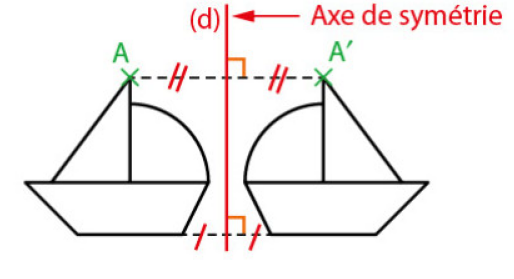
\includegraphics[scale=.5]{fig1}
		\end{center}	
	\end{myex}


\end{frame}

\begin{frame}
	
	\begin{columns}
		\begin{column}{0.35\textwidth}
			%\begin{left}
				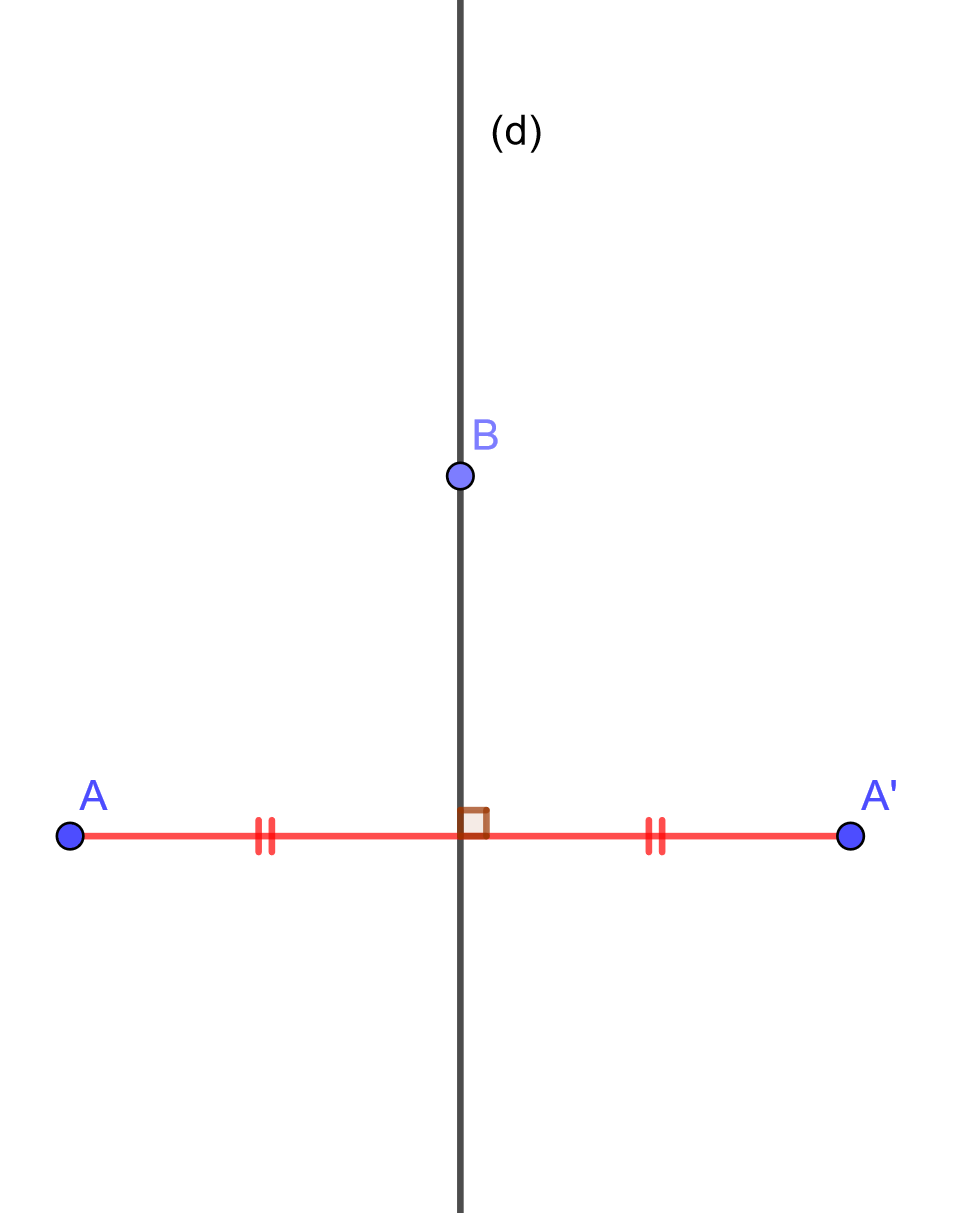
\includegraphics[scale=0.18]{def}
			%\end{left}
		\end{column}
	
		\begin{column}{0.65\textwidth}
			\begin{myprops}
				Soit $(d)$ une droite :
				\begin{itemize}
					\item Si un point $A$ n'appartient pas à la droite $(d)$, alors son symétrique par rapport à la droite $(d)$ est le point $A'$ tel que \kword{$(d)$ est la médiatrice du segment $[AA']$}.
					\item Si un point $B$ appartient à la droite $(d)$, alors son symétrique par rapport à la droite $(d)$ est \kword{lui même}.
				\end{itemize}
			\end{myprops}
		\end{column}
	\end{columns}
	
	
\end{frame}

\section{Symétrie centrale}


\begin{frame}
	\begin{mydef}
		
		Deux figures sont \kword{symétriques par rapport à un point $O$} si elles se superposent lorsqu'on effectue un demi-tour autour du point $O$. Le point $O$ est appelé \kword{centre de symétrie}.\pause
		
	\end{mydef}
	
	\begin{myex}
		\begin{center}
			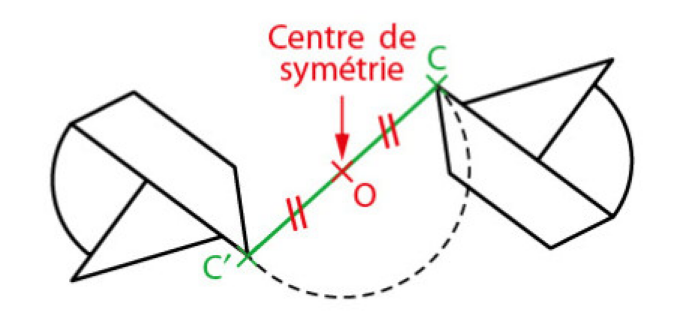
\includegraphics[scale=.5]{fig2}
		\end{center}
	\end{myex}
\end{frame}


\section{Propriétés de la symétrie}

\begin{frame}
	\begin{myprops}
		\begin{itemize}
			\item Le symétrique d'une droite par rapport à une droite ou un point est une autre droite. La symétrie \kword{conserve l'alignement}.
			\item Si deux droites sont \kword{symétriques par rapport à un point} alors elles sont \kword{parallèles}.
		\end{itemize}
	\end{myprops}
\end{frame}

\begin{frame}
	\begin{myexs}
		\begin{columns}
			\begin{column}{0.5\textwidth}
				
			
			\begin{center}
				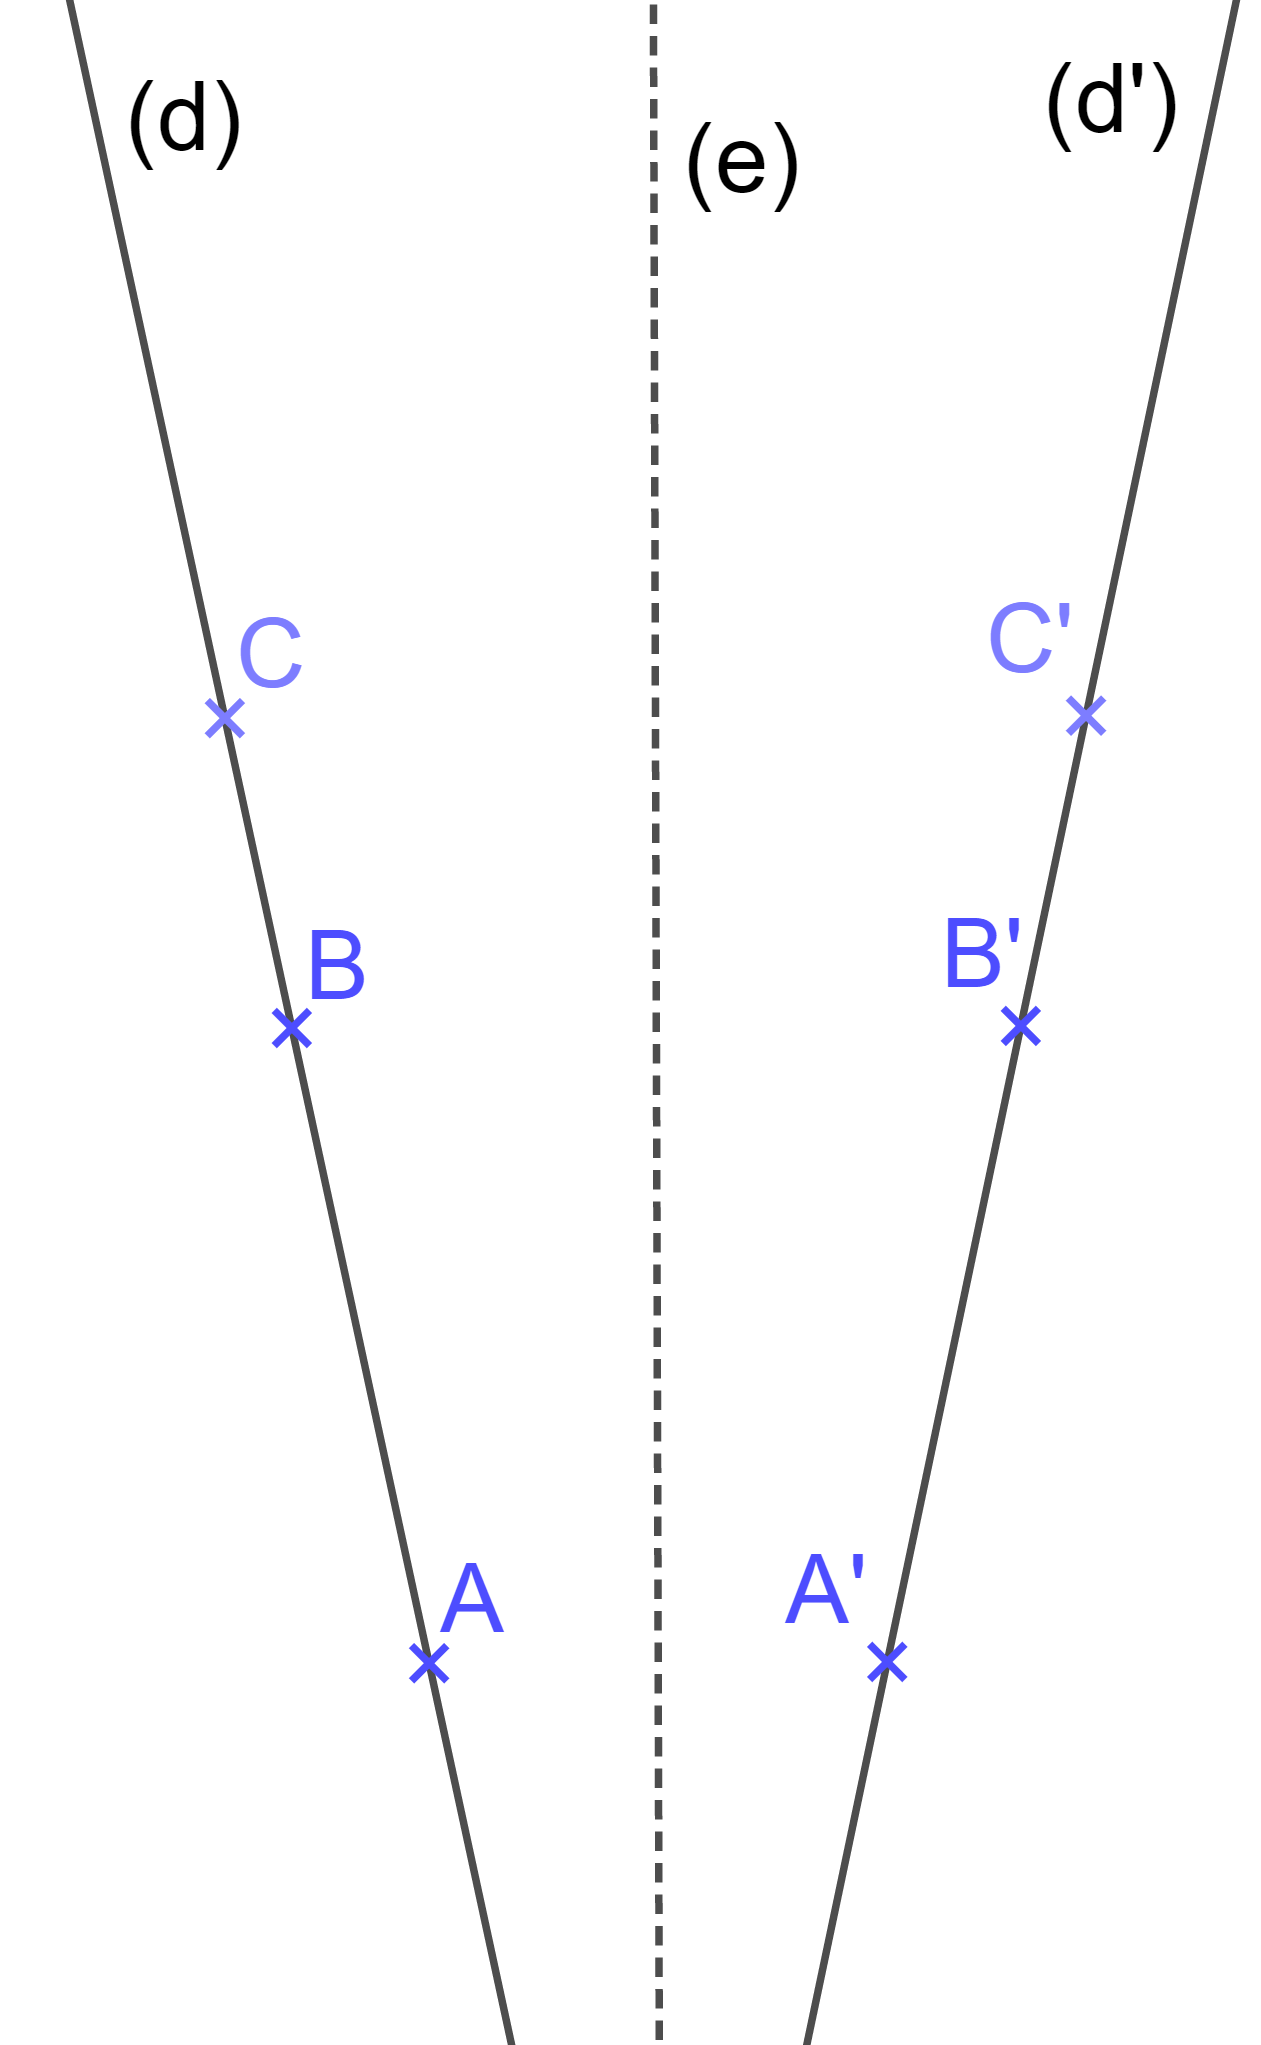
\includegraphics[scale=0.075]{sym_droites1}
			\end{center}
			
			\begin{itemize}
				\item Les points $A$, $B$ et $C$ sont alignés, donc $A'$, $B'$ et $C'$ leur symétriques par rapport à la droite $(e)$ sont \pause aussi alignés.
			\end{itemize}	
			
			\end{column}
		
			\begin{column}{0.5\textwidth}
			\begin{center}
				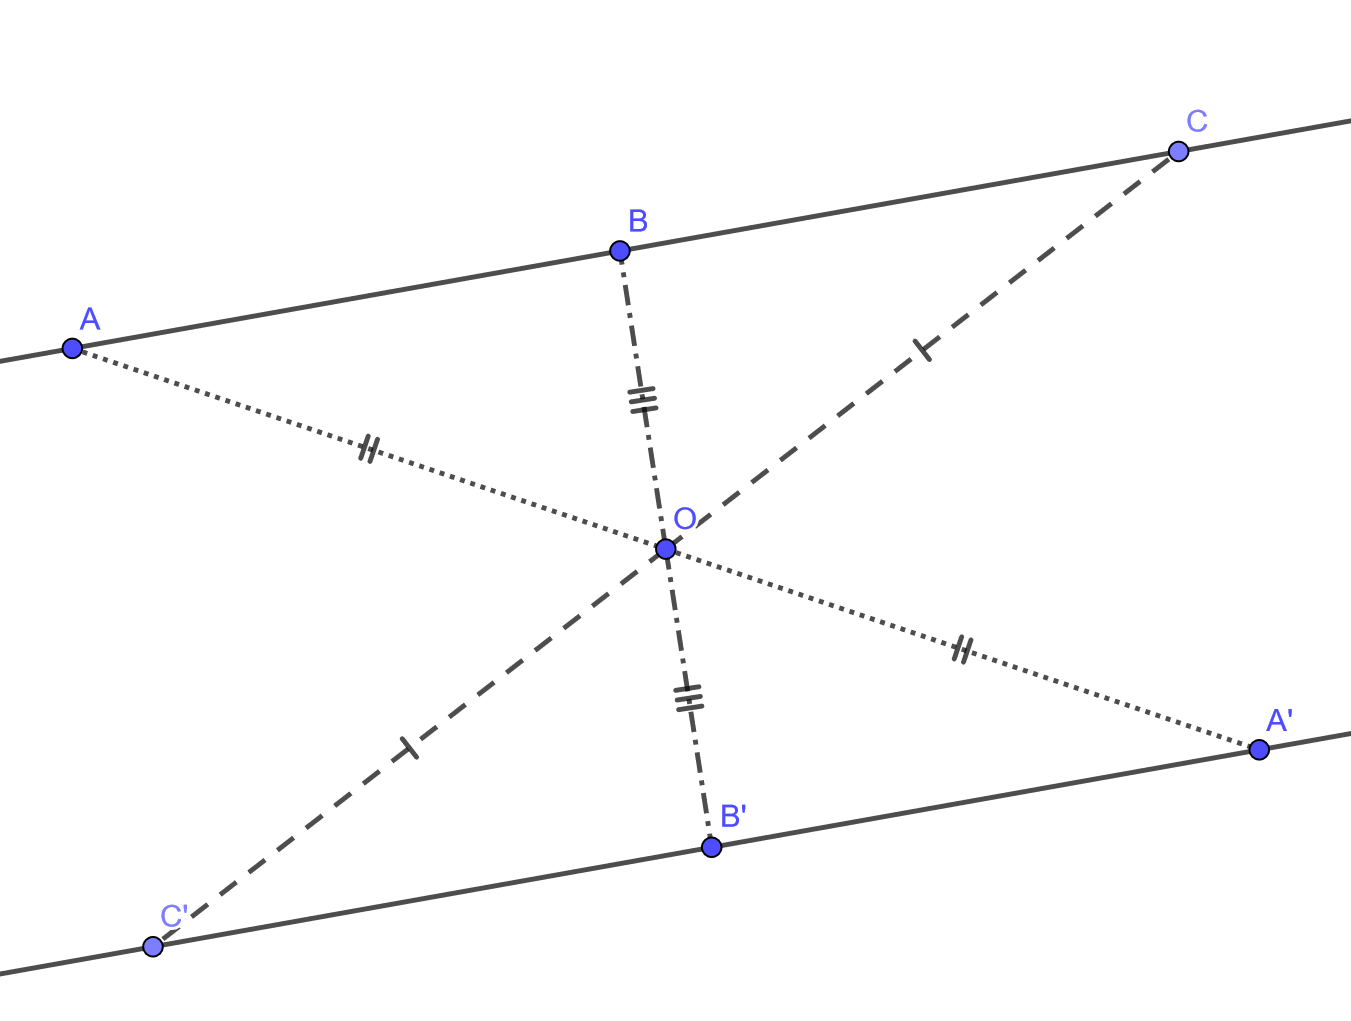
\includegraphics[scale=0.15]{sym_droites2}\pause
			\end{center}
			
			\begin{itemize}
				\item Les points $A$, $B$ et $C$ sont alignés, donc $A'$, $B'$ et $C'$ leur symétriques par rapport à la droite $(e)$ sont aussi alignés.\pause
				\item La droite $(AB)$ est parallèle à la droite $(A'B')$.
			\end{itemize}
			\end{column}
		\end{columns}
	\end{myexs}
\end{frame}

\begin{frame}
	\begin{myprop}
		Le symétrique d'un segment par rapport à une droite ou un point est un segment de \kword{même longueur}. 
	\end{myprop}
	
	\begin{myex}
		\begin{center}
			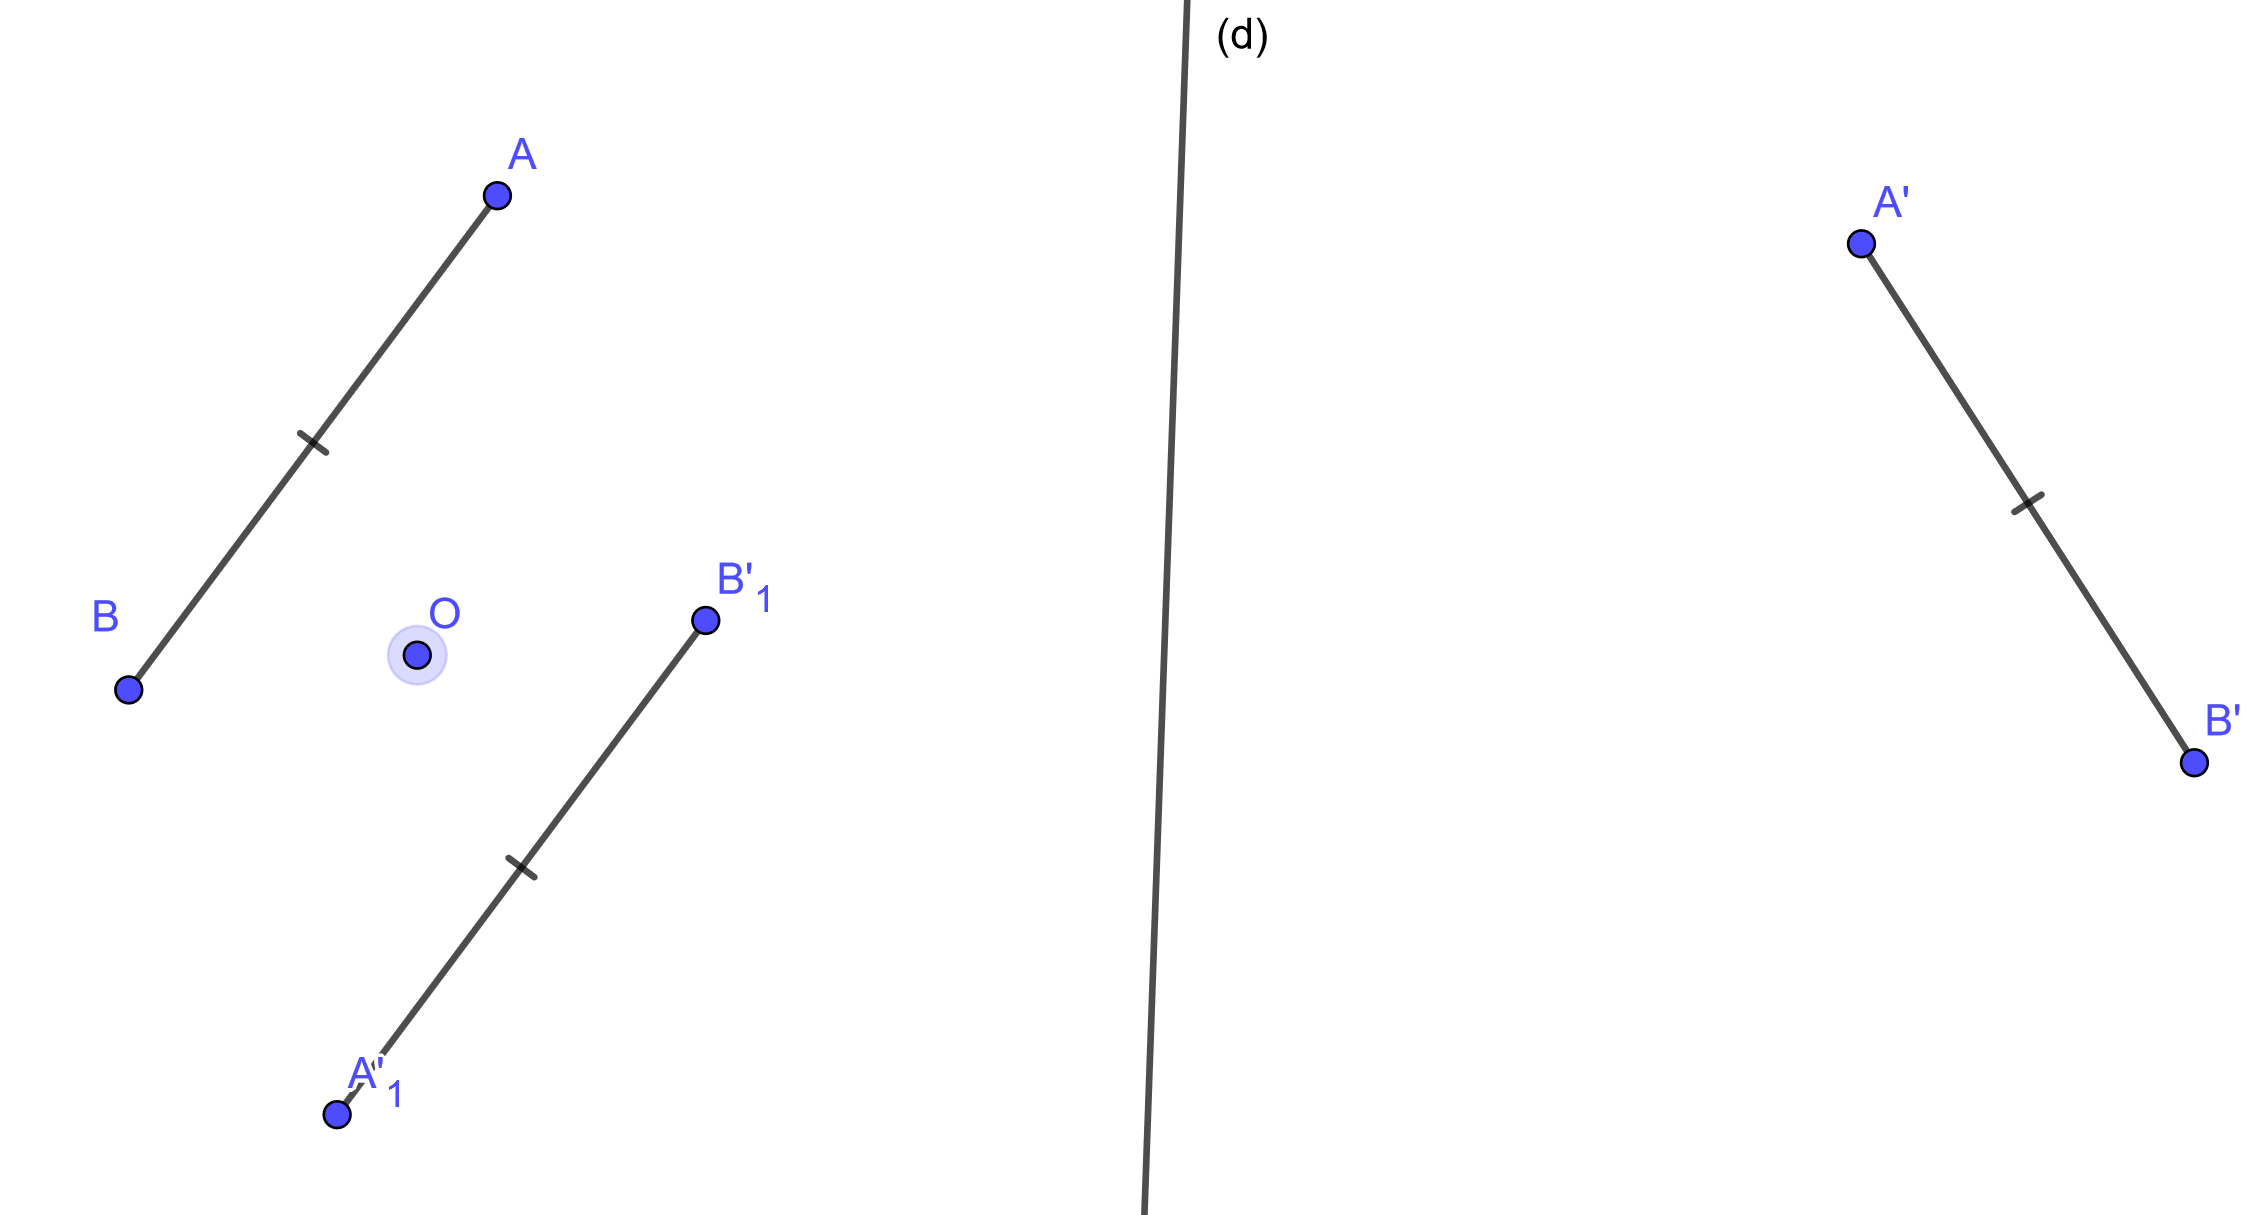
\includegraphics[scale=0.12]{sym_seg}
		\end{center}
		
		Le segment $[A'B']$ est le symétrique du segment $[AB]$ par rapport à la droite $(d)$ et $[A'_1B'_1]$ le symétrique de $[AB]$ par rapport au point $O$. \pause
		Ils ont tous la même longueur
		
		
	\end{myex}
\end{frame}

\begin{frame}
	\begin{myprop}
		Le symétrique d'une figure par rapport à une droite ou un point est une figure de même forme. La symétrie \kword{conserve les angles, les périmètres et les aires}.\pause
	\end{myprop}
	
	\begin{myex}
		\begin{center}
			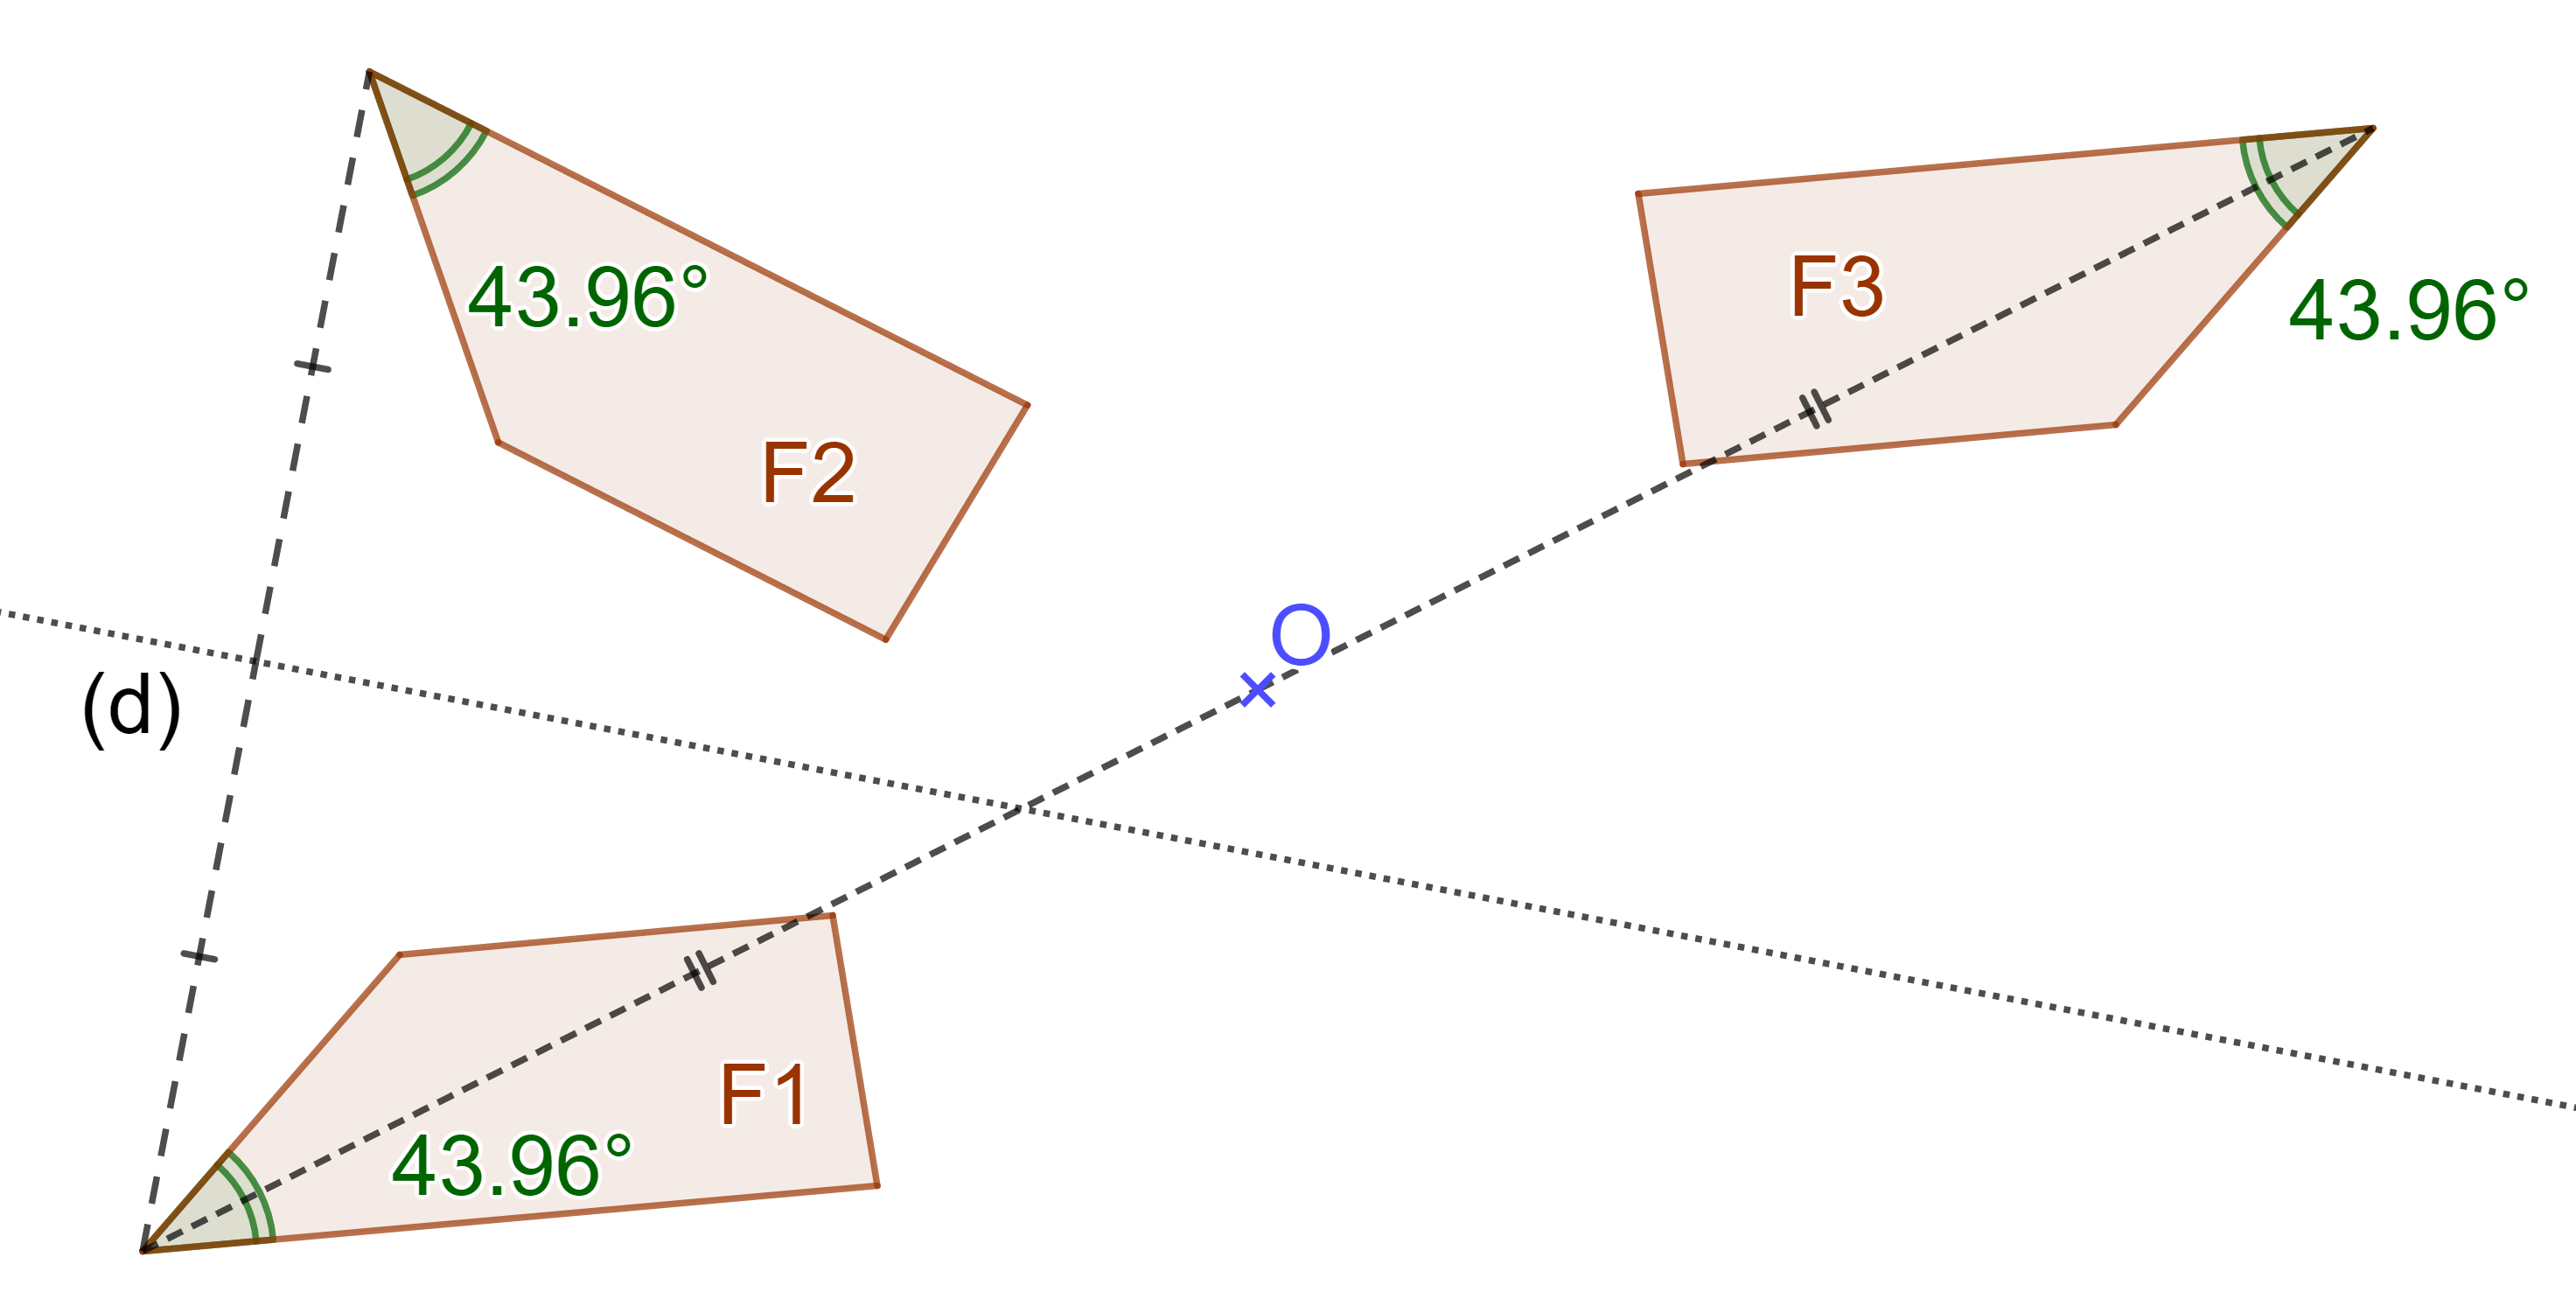
\includegraphics[scale=0.11]{sym_figures}
		\end{center}
		
		La figure $F2$ est le symétrique de $F1$ par rapport à la droite $(d)$; $F3$ est le symétrique de $F1$ par rapport au point O.\pause
		Elles ont le même périmètre, la même aire et leurs angles ont la même mesure.
	\end{myex}
\end{frame}
\end{document}